%Hasta el momento se detallaron las motivaciones del trabajo. Es decir, la necasidad de una comunicación de mayor ancho de banda que UART y que sea facil de transferir a una PC.
%Además de esto, se desarrolló la norma USB, seleccionada para implementar la comunicación
La implementación de la comunicación entre le FPGA y la PC, en este trabajo, se efectúa a través de USB 2.0. Para establecer esta comunicación, como se menciona en la Sección \ref{int:pro}, se utiliza una interfaz que ejecute las tareas relativas al protocolo, la transmisión y recepción de los datos.\\

La figura \ref{fig:etp} muesta en lineas de trazos tres partes principales en las que este trabajo descompone el problema: La comunicación entre el FPGA y la interfaz, la configuración de la interfaz misma y la conexión entre la PC y la interfaz. El desarrollo de cada etapa cuenta con herramientas específicas que facilitan en gran medida la tarea que se realiza. En este capítulo se detalla por separado las características de cada una de estas herramientas.\\
%Se puede descomponer la implementación en tres partes bien definidas: La comunicación entre el FPGA y la interfaz intermedia, la configuración de la interfaz misma, y la conexión entre la PC y la interfaz. El desarrollo de cada una de estas etapas contará con herramientas específicas.\\
%TODO: agregar una figura que muestre lo dicho en estos dos párrafos
\begin{figure}
	\centering
		\begin{tikzpicture}[]
			\begin{scope}[transform shape,node distance=1,>=latex]
				\node[rectangle, rounded corners,draw=black,minimum size=40](memo){Memoria};
				\node[](aux01)[right=of memo]{};
				\node[align=center,](comFIFO)[above=of aux01]{Comunicacion\\Interfaz - FPGA};
				\node[exterior](fpga)[right=of aux01]{FPGA};
				\node[rectangle, rounded corners, draw=black, minimum size=40,align=center](trans)[left=of memo]{Transceptor\\USB};
				\node[node distance=.5](aux02)[left=of memo]{};
				\node[](interfaz)[below=of aux02]{Interfaz};
				\node[](aux03)[left=of trans]{};
				\node[align=center](comPC)[above=of aux03]{Comunicación\\PC - Interfaz};
				\node[exterior](pc)[left=of aux03]{PC};
				\draw[thick,<->] (fpga) to (memo);
				\draw[thick,<->] (pc) to (trans);
			\end{scope}
			\begin{scope}[]
				\node[rectangle, dashed, draw=black, rounded corners, fit={(fpga)(memo)(comFIFO)}] (parte1) {};
				\node[exterior,fit={(trans)(interfaz)(memo)}](bridge){};
				\node[rectangle, rounded corners, dashed,draw=black, fit={(trans)(pc)(comPC)}](parte3){};
				\node[rectangle, rounded corners, dashed,draw=black, fit={(interfaz)(bridge)}](){};
			\end{scope}
		\end{tikzpicture}
		\caption{Partes en que se desglosa el trabajo}
		\label{fig:etp}
\end{figure}

%El objetivo que persigue el presente trabajo es el desarrollo e implementación de una comunicación entre una PC y desarrollos científicos basados en FPGA mediante el protocolo USB 2.0 de alta velocidad.\\
%
%Todo sistema USB puede se dividido en, al menos, tres etapas fundamentales que cumplen funciones específicas a lo que el protocolo se refiere. Estas tres etapas se observan en la Figura \ref{usbDeviceScheme}.\\
%
%De izquierda a derecha, la primera de ellas, el transceptor, se encarga de adecuar los valores de tensión, las frecuencias, impedancias y todo lo relacionado a las señales que envía el protocolo a través de sus conectores. el segundo, el Motor de Interfaz Serial (MIS), es el encargado de recibir los datos que se producen en el dispositivo, colocar el encabezado y la cola del mensaje, ordenar y armar los paquetes de forma tal que sean coherentes con el protocolo. También se encarga de recibir los paquetes que llegan por el bus, decodificarlos, corroborar que no presente errores y entregarlos al resto del dispositivo. Finalmente, la lógica de control es la encargada de enviar las ordenes de trabajo al MIS, producir y consumir los datos que van y vienen por el sistema.\\
%
%\begin{figure}
%	\centering
%	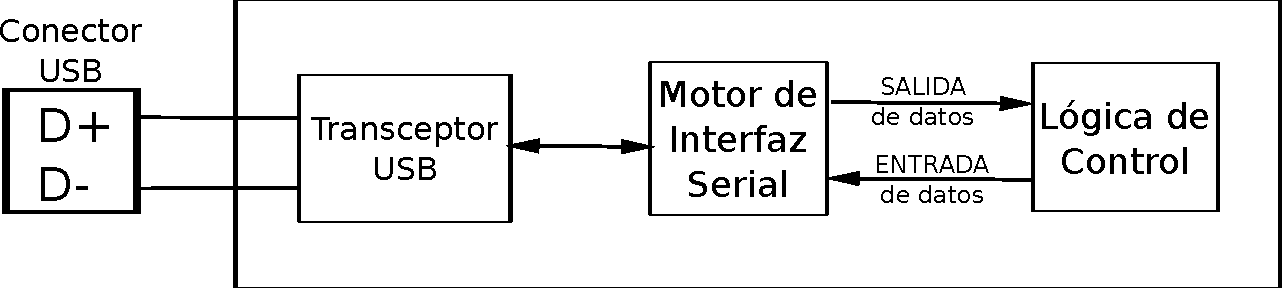
\includegraphics[width = 0.6\textwidth]{21sistemausb}
%	\caption{Etapas fundamentales de un dispositivo USB}
%	\label{usbDeviceScheme}
%\end{figure}
%
%Gracias al gran potencial que poseen los FPGA's, desde el punto de vista de la electrónica digital, es posible desarrollar en uno de estos dispositivos toda la lógica de control y el MIS. A los fines de la adecuación de las señales y todo lo relativo a la parte analógica del sistema, siempre será necesario un transceptor que se comunique con el bus. Esta implementación resulta minimalista desde el punto de vista de PCB y cantidad de CI necesarios.\\
%
%Sin embargo, este enfoque requerirá un gran consumo de recursos de una FPGA, los cuales son muy valiosos para realizar otro tipo de desarrollos y no para dedicarlos exclusivamente para la comunicación del sistema principal con una PC, presentando, en este sentido, ventajas mayores la utilización de otro tipo de trasnferencias.\\
%
%Es por esto, que se propone en su lugar, ocupar un integrado específico, diseñado para tal fin, y disponer de la mayor parte de los {\it slices} y bloques del FPGA para desarrollos complejos y complementarios. La Figura \ref{overview} muestra el esquema planteado, en donde se realiza dentro de la FPGA una maquina de estados algorítmica (MEA) mínima, que realiza un control mínimo del sistema y posee una aplicación que produce y consume datos; un controlador USB, que hace las veces de puente o interfaz entre el FPGA y una PC. Éste dispositivo posee el MIS y su control, los que se conectan a un trasceptor que el fabricante incorpora para los propósitos de la comunicación y buffers incorporados en donde almacena los datos que fluyen entre ambos extremos; finalmente, una PC que sirve para enviar y recibir datos, con el objetivo de corroborar el correcto funcionamiento de la comunicación.\\
%
%Como se explayará a continuación, para el bloque que corresponde a la FPGA, se utilizó un Spartan IV que viene integrado a una placa de desarrollo comercial que posee por nombre MOJOv3. La interfaz se implementa con un controlador USB CY7C68013A fabricado por Cypress Semiconductor, incorporado en una placa de desarrollo comercial CY3684 EZ-USB FX2LP Development Kit del mismo productor. En el lado de la PC, se utiliza la biblioteca de código abierto libusb-1.0, para elaborar una software escrito en lenguaje C que envie datos, los reciba y chequee los errores producidos.\\ 
%
%\begin{figure}
%	\centering
%	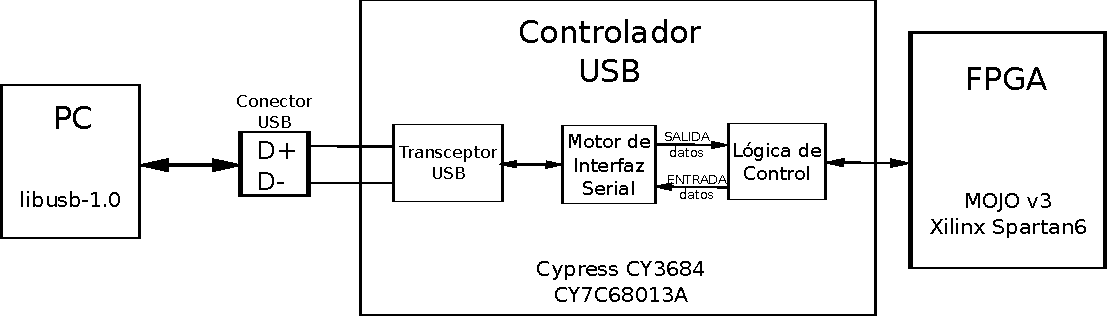
\includegraphics[width = 0.8\textwidth]{22overview}
%	\caption{Vista general del sistema propuesto}
%	\label{overview}
%\end{figure}